\chapter{Methods}
This section details the structured methodology employed to analyze Decentralized Autonomous Organizations, including the creation of a robust dataset, the implementation of a manual classification tool, the design of an LSTM model for activity prediction, and the development of heuristics for benchmarking the LSTM model.

\begin{table}[h]
\centering
\begin{tabularx}{\textwidth}{@{}l l X@{}}
\toprule
\textbf{Characteristic}       & \textbf{Input Feature}      & \textbf{Definition}      \\ \midrule
Monetary                      & US Dollar Price             & The daily price of one standard unit of the governance token, denominated in US dollars. E.g., the price if the governance token is denoted in Ether: 1 ETH $\approx$ 3,342.37 USD. \\
Social                        & $\Delta$ Twitter Followers  & The day-on-day change in the number of Twitter followers. If the account lost followers, the difference is represented by a negative integer.         \\
Technical                     & Development Activity        & A metric representing daily activity in the project's code repositories. Excludes unimportant activity like comments or forks. A detailed breakdown can be found on the Santiment documentation. \\ \bottomrule
\end{tabularx}
\caption{Description of Input Features}
\label{tab:input_features}
\end{table}

Having previously established all characteristics we need to analyze, we chose quantitative variables representing each of the characteristics.
Starting with the monetary characteristic, we settled on the price of the accompanying token of the DAO as a proxy variable.
Price reflects market sentiment and external perceptions of the DAO's performance or stability (\cite{rahman2018sentiment}). High or stable token prices indicate confidence in the DAO's governance and decision-making.

Regarding the social characteristic, we selected the daily change in Twitter followers of the project's Twitter profile. 
Twitter, in particular, is one of the most prominent platforms for engagement within the Web3 community (\cite{deepdao2022social}).
This serves as a proxy for community interest in the DAO for members and non-members alike.

Last but not least, we use a predefined development activity indicator by Santiment. This metric tracks GitHub contributions within the DAO's GitHub organization and accumulates them, excluding non-directly related activities such as comments on pull requests or the creation of forks. GitHub, with 85\% market share, is the largest source code management platform worldwide, hosting almost the entirety of Web3 projects like Bitcoin and Ethereum exclusively, making it sufficient as the only development activity input.

\section{The Dataset}
Having established all variables, this section focuses on the construction of a suitable dataset to test our hypothesis.
We would have liked to compare our model to CoinGecko's classification, but whenever their project was classified as inactive, tracking for all metrics regarding the project was stopped.
Therefore, we chose the Santiment Database\footnote{\href{https://santiment.net}{https://santiment.net}} for our experiment. It is the biggest collection of DeFi projects with sufficient metadata to conduct our research. 
As of September 25, 2024, the database contains a total of 3,420 projects. While the list of project names is freely available, we needed to heavily utilize their Application Programming Interface to access the time series data of each project.
After fetching all projects, only 3,413 projects had the required time series data to answer our research question (change in Twitter followers per day, price in USD per day, and development activity per day).
Similar to CoinGecko, Santiment does not exclusively list DAOs but rather Web3 projects of any kind.
Taking BNB Chain as an example, which is held by a traditional corporation rather than a DAO, is still tracked by Santiment.
To filter out all irrelevant projects, we cross-referenced all Santiment project tickers with Snapshot symbols using a custom script.
Snapshot\footnote{\href{https://snapshot.box}{https://snapshot.box}} is an off-chain voting platform where DAO projects can create spaces to let their members vote.
We could then be sure that each match fulfills all of the characteristics of a DAO as outlined previously. Specifically, as every project tracked by Santiment comes with its own token, each of the remaining projects must have a monetary, social, and technical characteristic. Therefore, we were able to classify all matching projects as DAOs.
After comparing project slugs, 1,396 projects or 41\% of all projects remained.
Cutting out all DAOs where the minimum time series duration was not subceeding 60 days in any of the categories, 1,332 projects remained.
Last but not least, the dataset was then split into a training dataset consisting of 1,066 DAOs (80\%) and a test dataset containing 266 observations (20\%).

\begin{figure}
    \centering
    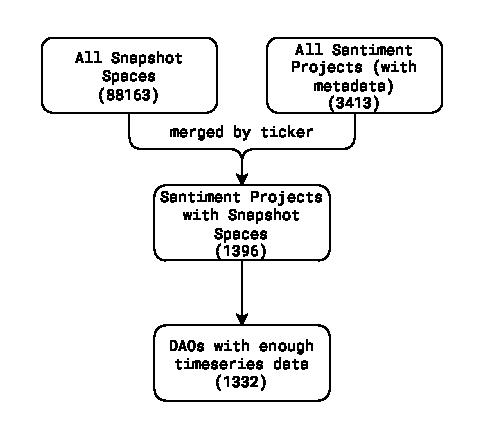
\includegraphics[]{assets/preprocessing_pipeline.pdf}
    \caption{Flowchart of preprocessing steps.}
    Number of remaining samples in parentheses.
    \label{fig:preprocessing}
\end{figure}

\section{The Manual Classification Utility Program}

After gathering our initial dataset, we required a method to manually classify the activity level of each DAO efficiently. Since this study is the first of its kind, no established tools were available. To address this, we developed a custom utility program to make the classification process less error-prone and more efficient.
The program features a straightforward four-panel dashboard, as shown in Figure \ref{fig:utility_program}, which presents data for each sample in the form of a line chart. A key feature of the dashboard is its ability to align all inputs on a unified timescale, even when time series data between its input features are inconsistent. For example, while the Ethereum Foundation’s Twitter account was created in January 2014, Santiment only began tracking its followers in 2018. The dashboard accounts for such discrepancies by automatically adding appropriate padding to the graph. The same normalization is applied to the development activity feature.
An additional quality-of-life improvement for human classifiers is the visualization of cumulative changes in Twitter followers.
While our decision models process raw day-over-day changes, cumulative data points make it easier for a person to observe trends.
Furthermore, the dashboard includes an interactive feature: hovering over the price graph displays a red dotted horizontal line at the cursor’s position, allowing the human classifier to annotate the activity state with a single click.
Once the user clicks, all data points before the selected time are automatically labeled as active, while those afterward are marked inactive.
This annotation process assumes a single transition from active to inactive, as no DAOs in our data set showed evidence of reactivation, making this simplification appropriate for the study.

\begin{figure}[h!]
    \centering
    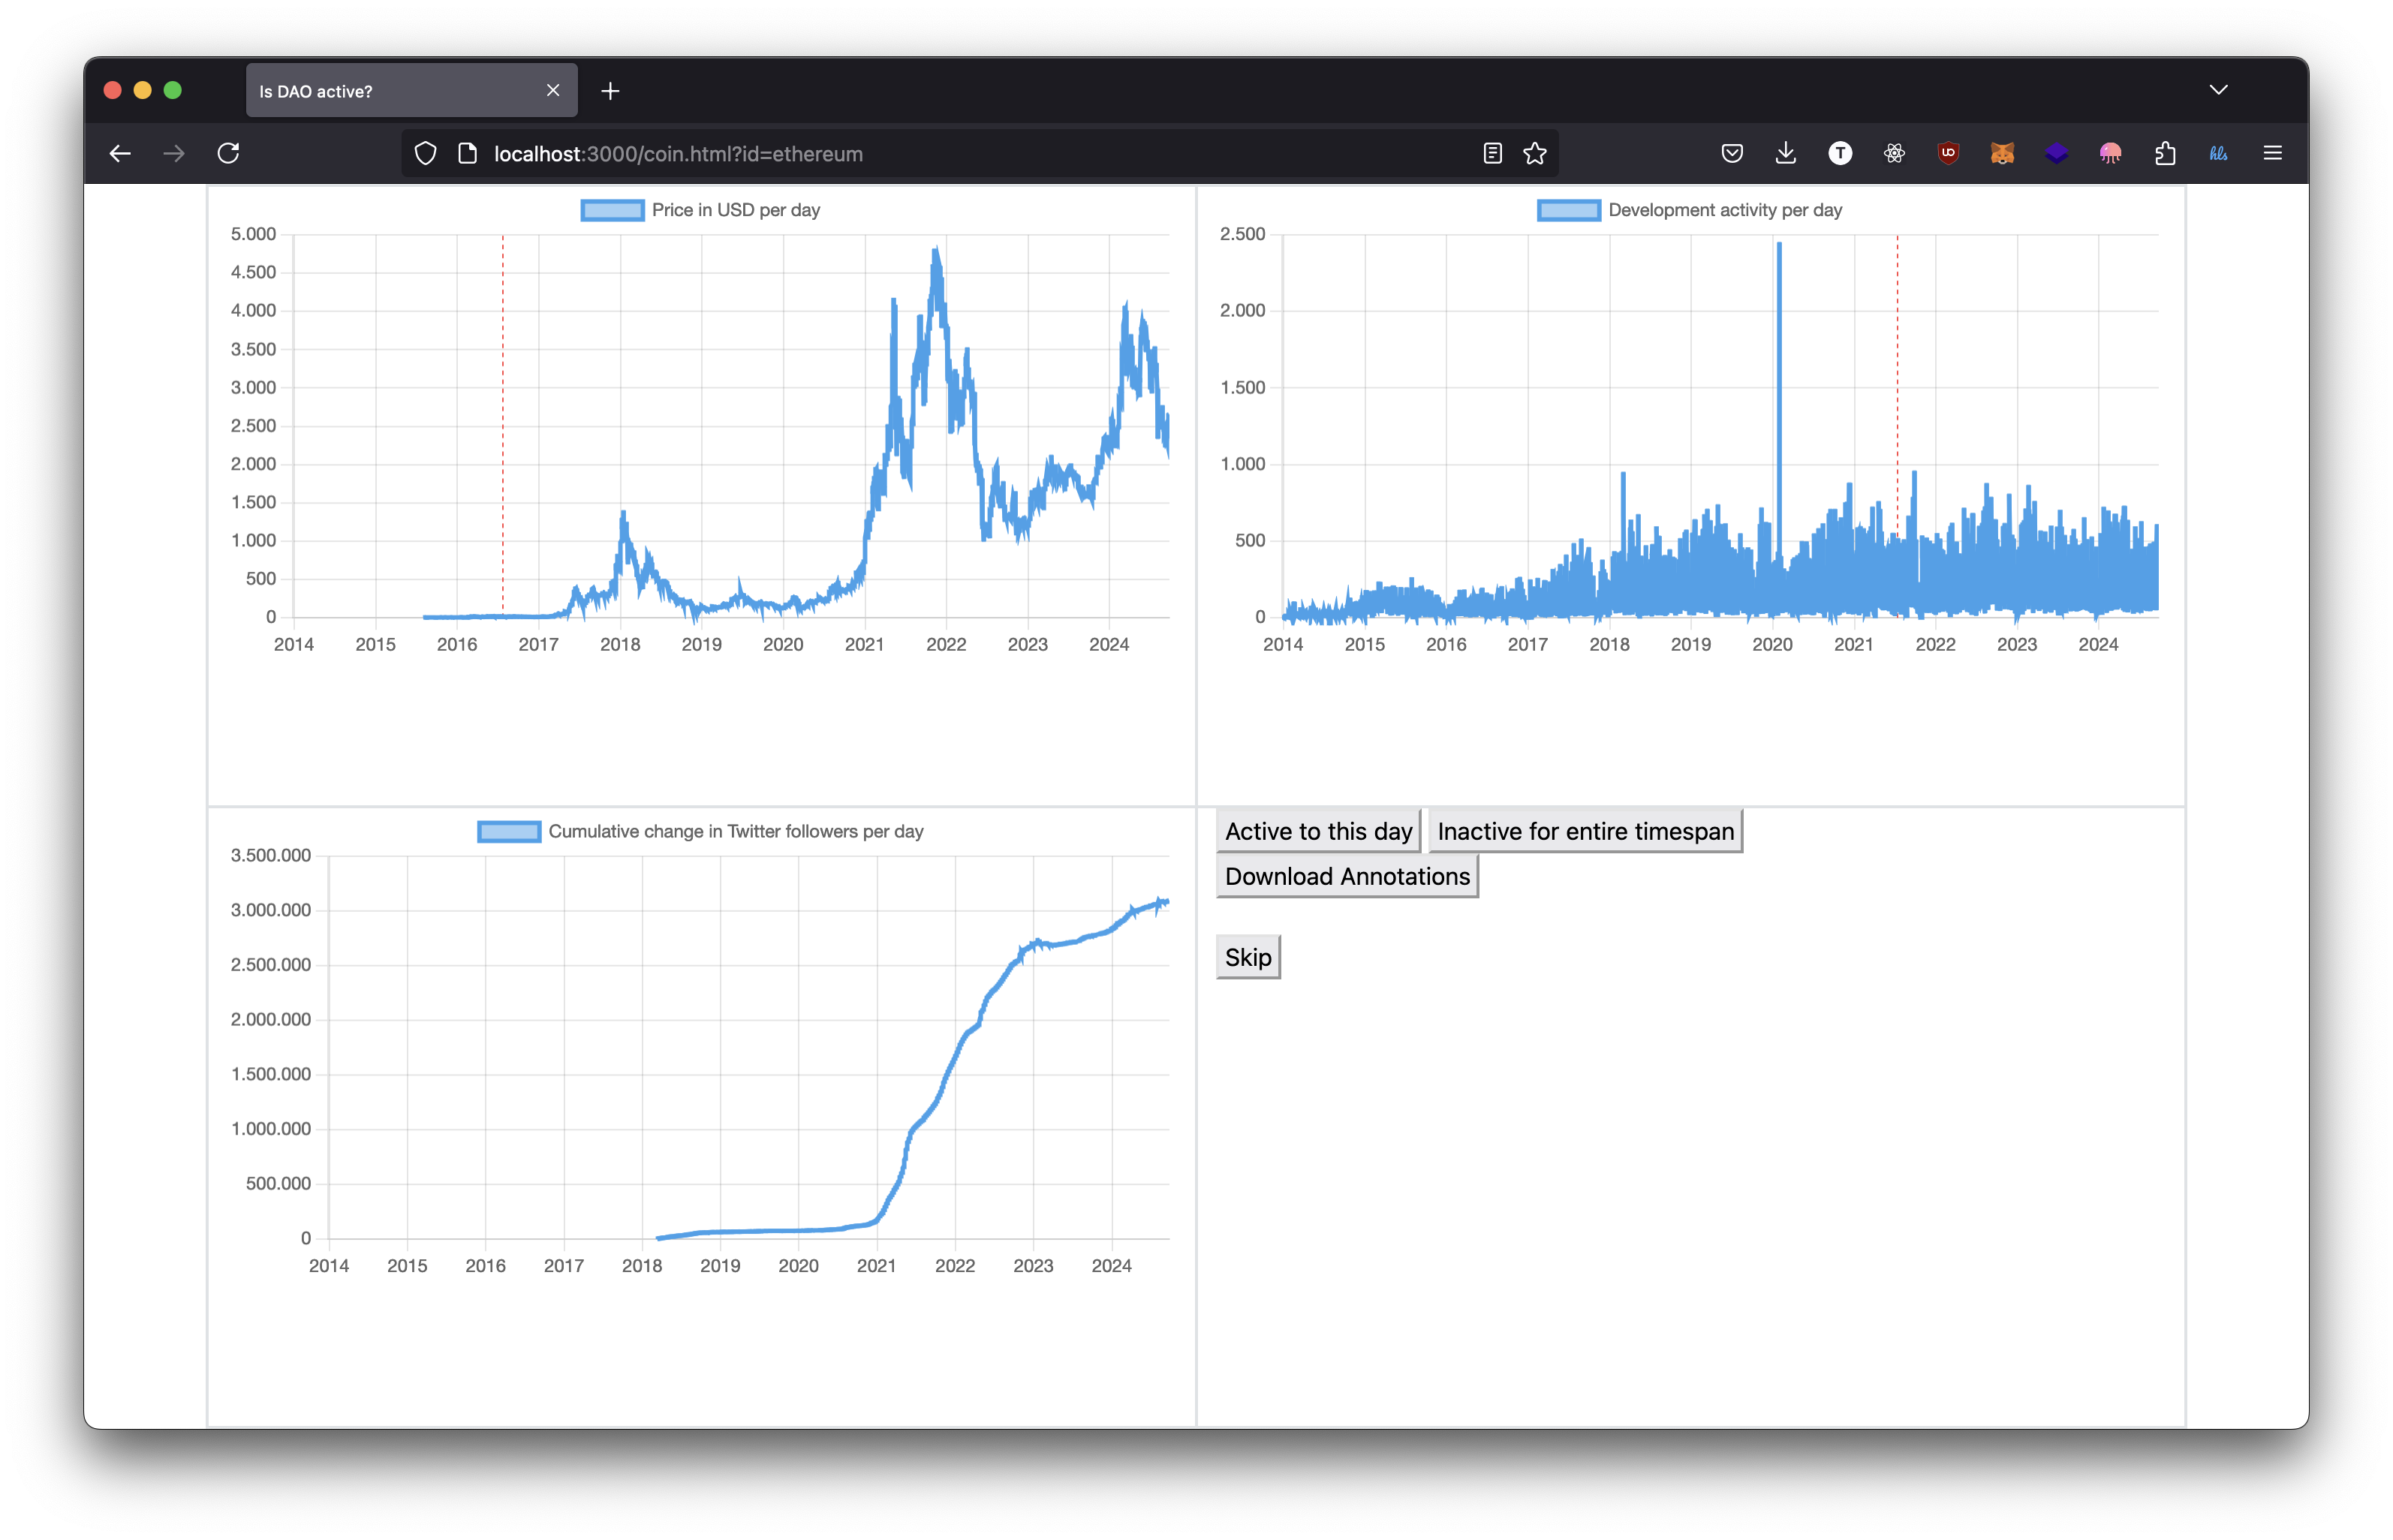
\includegraphics[width=\textwidth]{assets/util_screenshot.png}
    \caption{Screenshot showcasing the utility program.}
    \label{fig:utility_program}
\end{figure}

To support further research, we have open-sourced the program\footnote{\href{https://github.com/Throvn/bachelor-thesis}{https://github.com/Throvn/bachelor-thesis}}. The utility program is implemented in JavaScript and runs directly in a browser, providing a lightweight and accessible solution for DAO classification. We successfully used this program to manually classify the activity levels of all 1,332 DAOs in the dataset.

\section{The LSTM Model}

For the classification of the labeled data, we chose to utilize a Long Short-Term Memory (LSTM) network.
LSTMs are a specialized type of Recurrent Neural Network (RNN) designed to handle sequential data and interdependent inputs, making them well-suited for multivariate time series applications like ours.
Although our application relies exclusively on past inputs, we opted for a bidirectional LSTM setup.
This configuration, which processes inputs in both forward and backward directions, is known to reduce overfitting and improve generalization compared to unidirectional models.
Empirically, we observed that the bidirectional model performed slightly better in our tests, further validating our choice.
We also incorporated dropout layers during training to prevent overfitting due to the large number of parameters (\cite{srivastava2014dropout}).
This regularization technique improves the model's ability to generalize by randomly deactivating connections.
Our model processes three inputs as a time series. The input layer is shaped as $(T, 3)$, where $T$ represents the length of the time series. Each input must have a minimum length of 60, with each entry corresponding to one day. Thus, a DAO must exist for at least 60 days before its activity can be predicted.
The inputs are passed through an LSTM layer containing 128 neurons. To prevent overfitting, the outputs are then fed into a dropout layer, where 50\% of the neurons’ weights are set to zero. For computational efficiency, the activation function is applied after the regularization layer\footnote{https://sebastianraschka.com/faq/docs/dropout-activation.html}. We use a Rectified Linear Unit (ReLU) activation function to introduce non-linearity, allowing the model to capture more complex patterns.
This sequence of layers is repeated, with the only difference being a reduced dropout rate of 30\%. The resulting outputs are fed into a fully connected layer with a single neuron, which predicts the DAO's activity level. Last but not least, a sigmoid function is applied to ensure the output is bounded between zero and one, representing the activity level as a percentage.
The architecture can also be seen in Figure \ref{fig:lstm_architecture}.
\begin{figure}
    \centering
    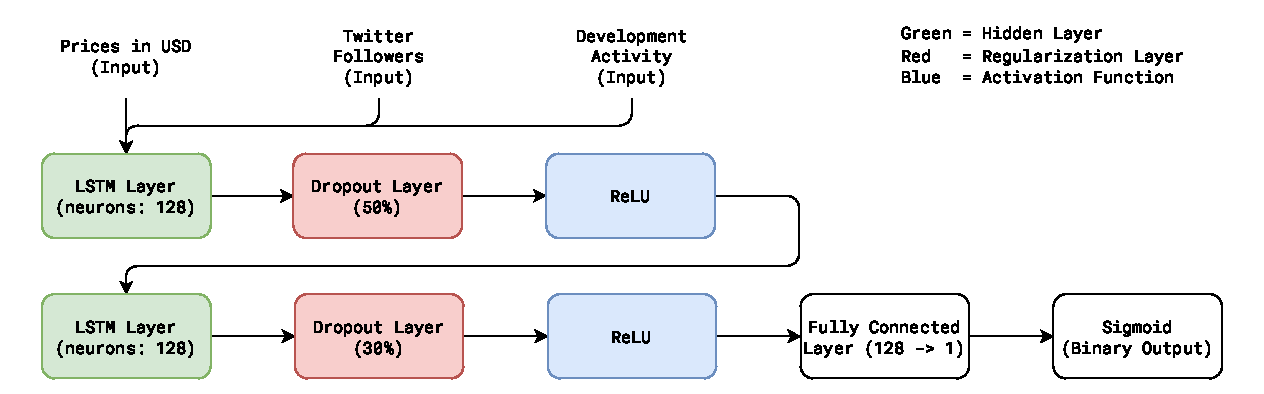
\includegraphics[width=\textwidth]{assets/lstm_architecture.pdf}
    \caption{Diagram of LSTM Architecture.}
    \label{fig:lstm_architecture}
\end{figure}

The model was then compiled using the Adam optimizer and a focal loss function. 
The focal loss function modifies the standard cross-entropy loss to focus more on hard-to-classify examples by down-weighting the loss contribution of well-classified examples. It introduces two parameters, alpha and gamma. Alpha is a weighting factor that balances the importance of positive and negative classes, while gamma is a focusing parameter that reduces the loss for well-classified examples, emphasizing harder ones. 
The cross-entropy loss measures the difference between the true distribution and the predicted probability distribution. As a natural consequence, the model tries to minimize uncertainty between the two distributions.
This adjustment is particularly helpful in our imbalanced dataset where inactive data points make up only 21\% of the total, compared to 79\% for active data points.
By emphasizing the minority class, the focal loss function helps the model better capture patterns in underrepresented data.
The LSTM's temporal features were then fed into XGBoost, which refines predictions through gradient boosting, iteratively correcting errors.
This hybrid approach combines the LSTM's sequence modeling with XGBoost's adaptability to enhance classification performance.

The model was trained to predict the transition of a DAO from an active to abandoned activity level. Its output is the predicted probability of the DAO remaining active on the next day, attempting to identify both the occurrence and timing of the operational switch.
The input data for the model consists of the longest available time series where all input variables—USD price, changes in Twitter followers, and developer activity—have complete entries. Consequently, the model does not include controls for missing data and was never trained on incomplete records. To maintain temporal dependency in the dataset, we employed a time series split, enabling the model to generalize fresh inputs.
As LSTMs can accommodate nonlinear dependencies, the model processes changes in Twitter followers without the need for preprocessing, and normalization of inputs was also skipped due to the capabilities of LSTMs to manage unscaled data.
To compare the accuracy between experiments while minimizing computational costs, intermediate models were trained using a unidirectional architecture. Some experiments were undertaken by changing the parameters for the focal loss function. The best results were achieved by setting $\alpha = 0.71$ and $\gamma = 3$. However, the test pairs, among others, also included $(\alpha = 0.5, \gamma = 1)$ and $(\alpha = 0.71, \gamma = 2)$. Notably, a focal loss of $\alpha = 0.5, \gamma = 1$ equals the normal binary cross-entropy loss. The results can be seen in Table \ref{tab:alpha_gamma_comparison} of the Appendix.
After this initial experimentation, we decided to train a bidirectional model using the same parameters. While activity prediction realistically only happens from the past into the future, a sharp change in any of the inputs might make more sense when viewed in the context of both prior trends and future corrections.
The final model was trained on a MacBook Pro M2 with 16 gigabytes of RAM. Training the bidirectional model took about ten hours.

\section{The Heuristics}
To establish a baseline for comparison with our LSTM model, we selected simple heuristics based on individual DAO characteristics to evaluate the activity level of a DAO.
The first heuristic focuses on a DAO's Twitter following. By analyzing the cumulative daily change in followers, a positive or stable trend indicates growth and suggests the DAO is active. A declining trend, on the other hand, points to potential disputes or internal issues, increasing the likelihood of abandonment. One can therefore denote the activity level as a Heaviside step function where:
 \[
    {\text{activity level} = \left\{ \begin{array}{cl}
    0 & : \ x \leq 0 \\
    1 & : \ x > 0
    \end{array} \right.}
    \text{, where } x \text{ is the slope of the trend.}
\]
The second heuristic uses the same trend analysis but applies it to the price in US Dollars using raw pricing data, as -- unlike follower counts -- the price does not require accumulation. An increase in price indicates growing interest and participation in the DAO, as higher demand typically reflects greater engagement. Since every DAO starts as an active entity, a rising price supports the assumption that the DAO remains active.
The third heuristic assesses development activity, acknowledging that the size of development teams is generally stable or changes slowly, a trend heuristic would not make sense. Even a small, steady development team can indicate an active DAO. Therefore, for this heuristic, inactivity is defined as the absence of development activity over the past two weeks. This criterion ensures that consistent but low-level development still qualifies a DAO as active. We chose the interval of two weeks as this seemed like the best trade-off between timely results but also accounted for scheduled development breaks like holidays or weekends.

In this chapter, we discussed the dataset used to train and test our central hypothesis, as well as the manual classification tool for annotating the data. We then explained the structure of the LSTM model designed to validate the hypothesis and outlined alternative benchmarks for comparison. In the next chapter, we will present the results of the models introduced here.